\chapter{METHODOLOGY}
\hspace{\parindent} 
This section describes the methodology for developing the smart companion system for elderly care. The methodology comprises system design, data collection, pre-processing techniques, machine learning methods, hyperparameter configurations, and performance evaluation. The technical methods used in this study include speech recognition, natural language processing, sentiment analysis, and real-time video intercommunication. Each stage of the methodology is explained to ensure clarity and reproducibility.


\section{System Design}
\noindent\hspace{2.2em}The proposed smart companion system is designed to support elderly care by combining emotion recognition, real-time communication, and health monitoring. The system architecture consists of hardware (lightweight client), software application, and database components that collectively deliver personalized assistance. The functional diagram of the system is illustrated in Figure 3.1.

\begin{figure}[!htbp]
    	\centering
    	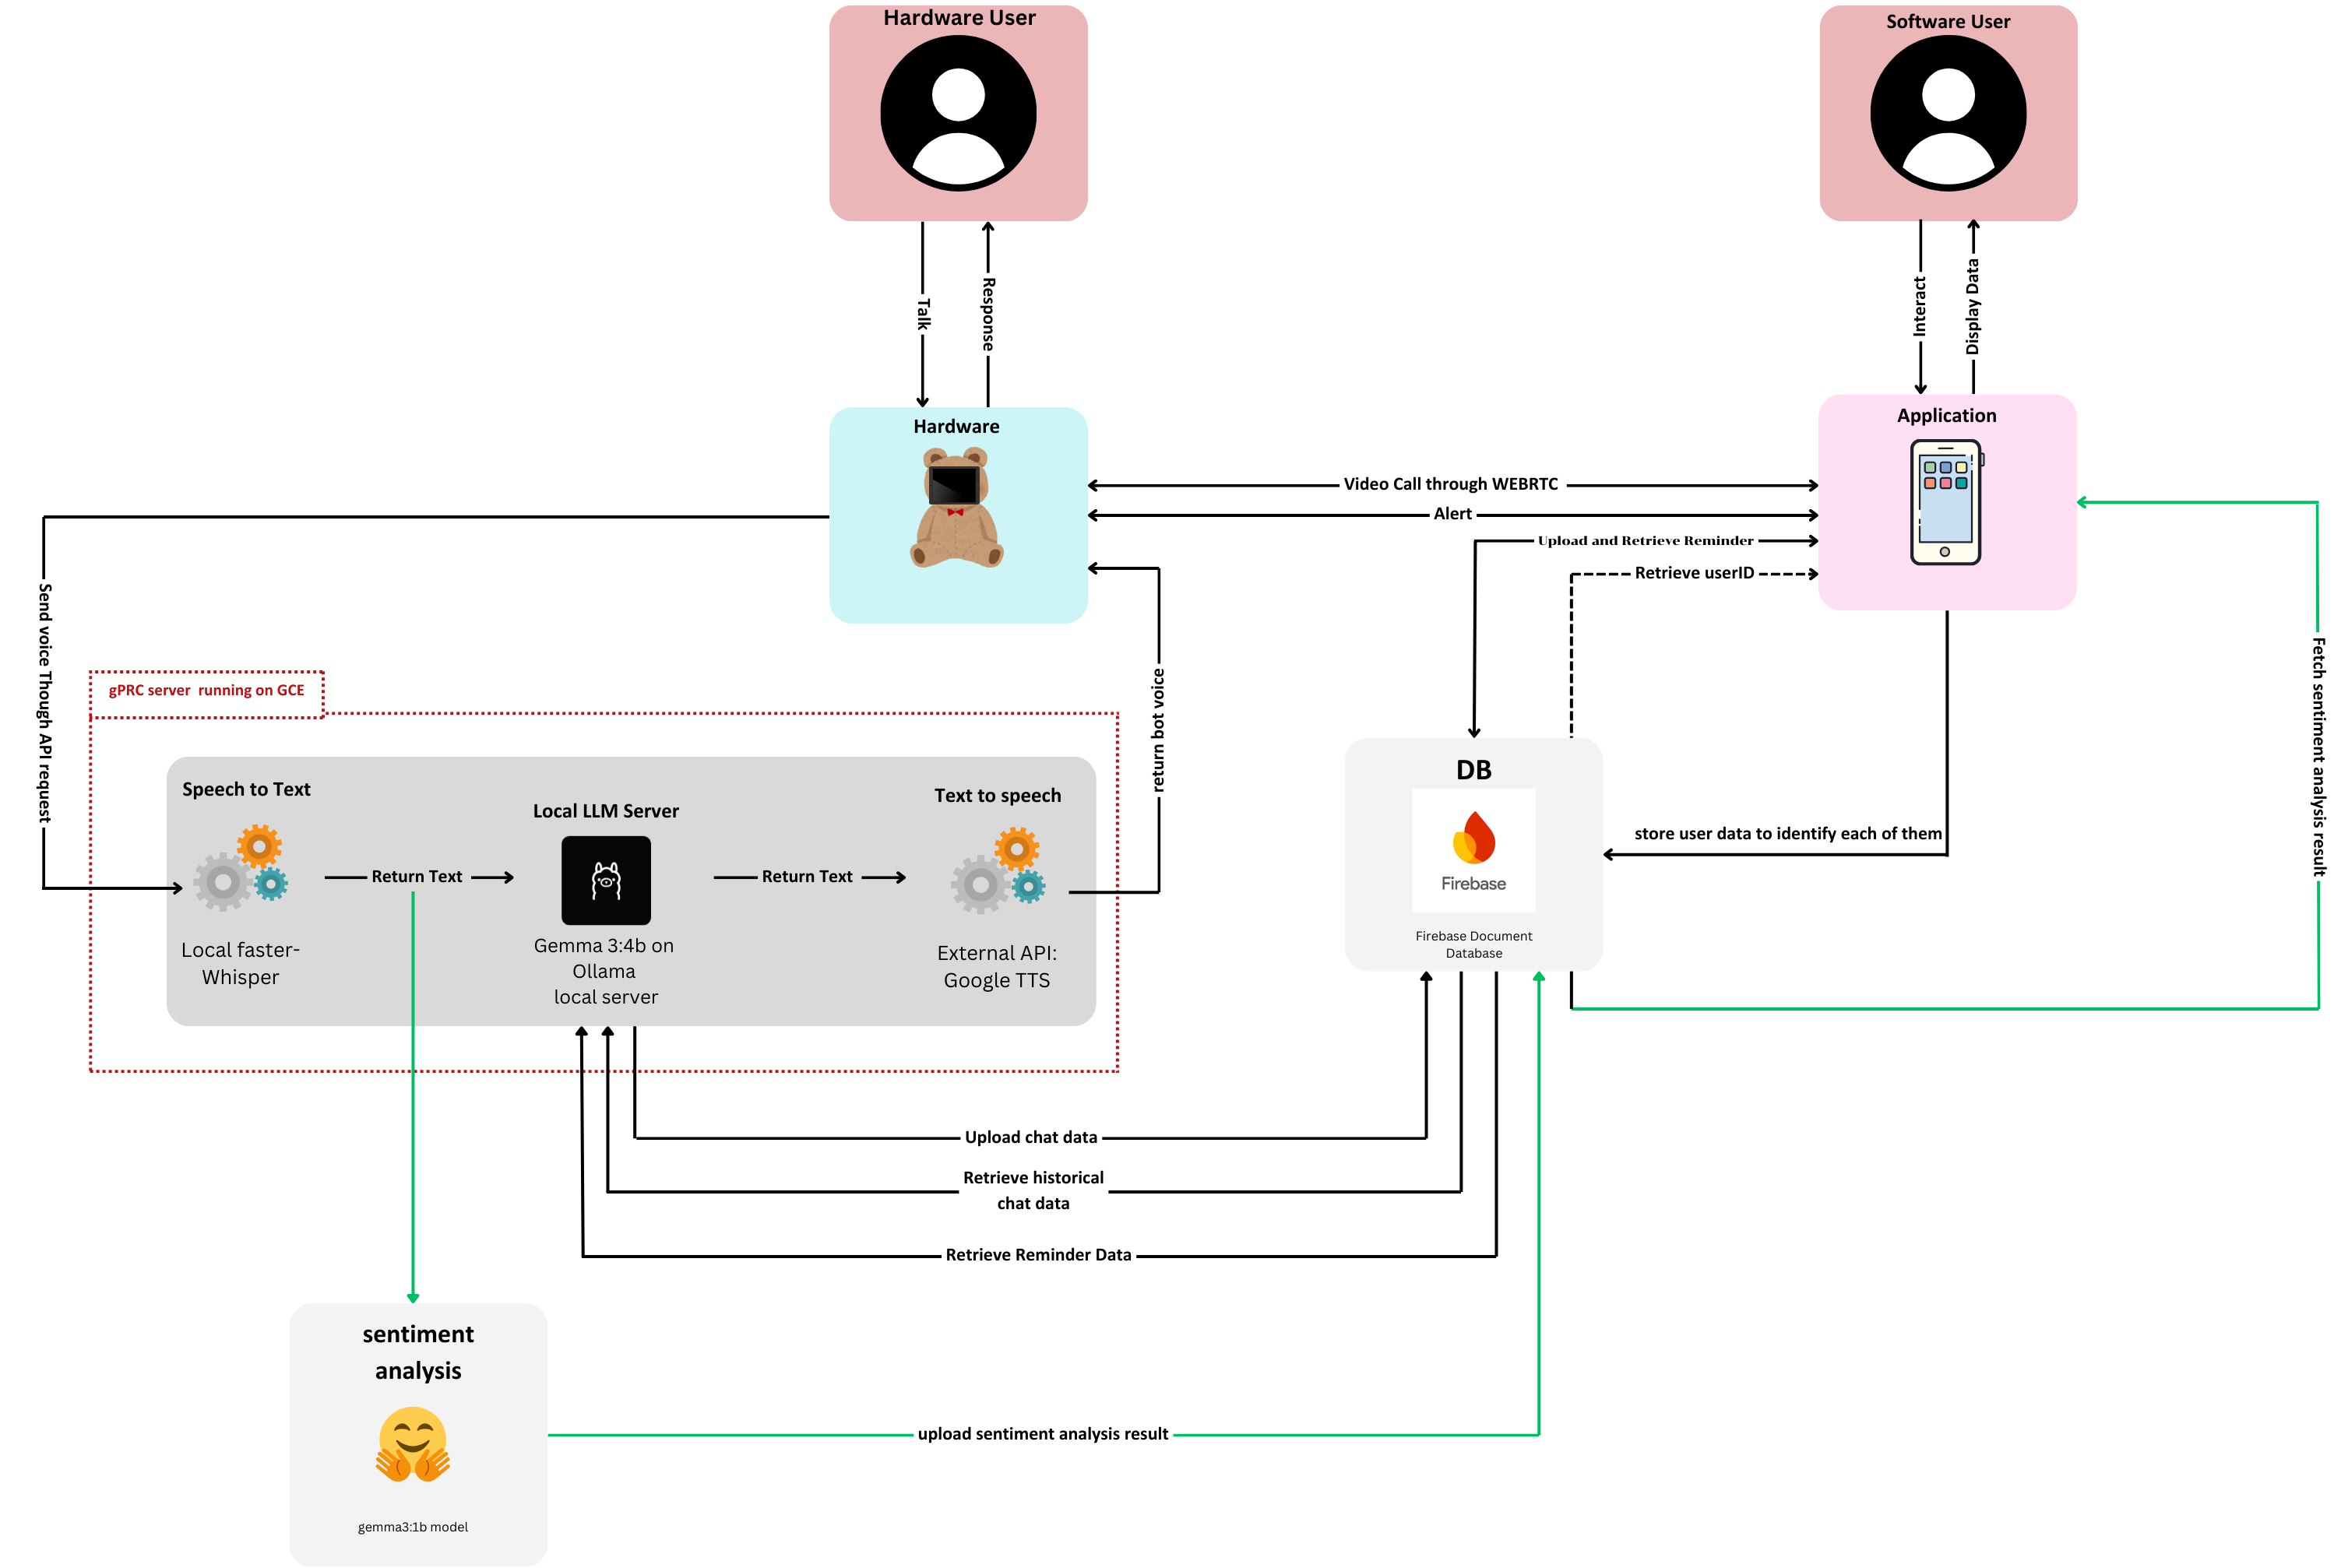
\includegraphics[width = 0.99\textwidth]{figures/BuddySystemFlowPic.png}
    	\caption{\textbf outlines the interaction between elderly application, caretaker application, and backend services. The elderly application acts as the primary interaction device, capturing voice and projecting chatbot voice response.}
    	\label{fig:paragraph}
\end{figure}
\FloatBarrier

\noindent\textbf{Key Components:}
\begin{itemize}
	\item Tablet Application: Captures speech and visual data.
	\item Mobile Application: Allows monitoring and communication with hardware users.
	\item Speech Recognition: Faster Whisper model for offline, high-accuracy Thai speech recognition.
	\item API Server: FastAPI server to handle tokenization and requests.
	\item Local LLM: GEMMA 3 for emotion classification and dialogue generation.
	\item Text-to-Speech: Google Text to Speech API converts the model responses into audio feedback.
	\item Video Call System: ZegoCloud SDK for stable, low-latency video communication.
	\item Database Systems: Firebase for user information, chat history, emotion history, reminder
\end{itemize}

\section{Data}
	\noindent\hspace{2.2em}The system relies on audio and visual data collected from elderly users during natural conversations. Audio data is captured using microphones embedded in the hardware client, while visual data is captured through cameras for real-time video communication. The collected audio data is processed for speech transcription, while text data is processed for emotion recognition and conversation generation.\\
\textbf{Data Processing}
\begin{itemize}
	\item Audio Transcription: Faster Whisper performs automatic speech recognition (ASR) to convert spoken Thai into text with high accuracy.
	\item Text Tokenization: Transcribed user inputs are tokenized and filtered (e.g., removing non-speech artifacts) before being processed by the LLM for emotion classification and response generation.
\end{itemize}


\section{Methods}
\noindent\textbf{Speech Recognition - Faster Whisper}\\
	\noindent\hspace{2.2em}Faster Whisper is a reimplementation of OpenAI's Whisper model using CTranslate2, designed for high-performance inference. It provides offline, accurate Thai speech recognition without relying on external cloud services. The process involves:
\begin{itemize}
	\item Audio Ingestion: Accepts raw audio streams from the hardware microphone.
	\item Voice Activity Detection (VAD): Uses WebRTCVAD to strictly filter non-speech audio.
	\item Feature Extraction: Converts audio to log-Mel spectrograms.
	\item Model Inference: Runs the `large-v3` model quantized to `int8\_float16` on the GPU for rapid transcription.
	\item Post-Processing: Ensures the output is valid Thai text.
\end{itemize}

\noindent\textbf{Emotion Recognition - GEMMA 3:1b}
\begin{itemize}
	\item Audio Emotion Recognition: GEMMA 3 model classifies the emotion from the converted texts.
\end{itemize}

\noindent\textbf{Dialogue Generation - GEMMA 3:4b}
\begin{itemize}
	\item The GEMMA 3 model generates emotionally-aware conversations by combining sentiment analysis and dialogue generation.
\end{itemize}

\noindent\textbf{Text-to-Speech - Google Text-to-Speech API}
\begin{itemize}
	\item Converts the generated text response into natural-sounding Thai speech using the Neural2 model (`th-TH-Chirp3-HD-Charon`) for a high-quality user experience.
\end{itemize}

\noindent\textbf{Video Call Communication - ZegoCloud}
\begin{itemize}
	\item ZegoCloud is used to facilitate stable, low-latency real-time video communication between elderly users and their family members, ensuring reliable connection even in fluctuating network conditions.
\end{itemize}

\noindent\textbf{Mood Summary Generation}
\begin{itemize}
	\item Mood Summary is summarized based on conversation data using GEMMA 3:1b and stored in Firebase database.
\end{itemize}

\noindent\textbf{Reminder System}
\begin{itemize}
    \item Caretakers can schedule reminders (e.g., for medication or appointments) through the mobile application. These reminders are synchronized with the backend and announced aloud by the chatbot to the elderly user at the designated time using the Text-to-Speech system.
\end{itemize}

\noindent\textbf{Caretaker Call Initiation}
\begin{itemize}
    \item The system allows elderly users to initiate a video call to their registered caretaker using a  voice command with intent to make a call (e.g., "Call grandchild"). Upon receiving the voice command, the chatbot facilitates the connection via the ZegoCloud SDK, enabling direct communication between the elderly user and their caretaker.
\end{itemize}


\section{ Database Schema}
	\noindent\hspace{2.2em} 
The system utilizes PostgreSQL for user-related data and MongoDB/Pinecone for emotion summaries and conversation as shown in Figure 3.2. The key database tables and collections are:\\
\textbf{PostgreSQL Database (User Data)}
\begin{itemize}
	\item \textbf{Users Table}
	\begin{itemize}
		\item user\_id (Primary Key, INT)
		\item name (VARCHAR)
		\item age (INT)
		\item email (VARCHAR)
	\end{itemize}
\end{itemize}

\noindent
\textbf{MongoDB (Emotion Summary Storage)}
\begin{itemize}
	\item \textbf{Emotion Summaries Collection}
	\begin{itemize}
		\item \_id (Primary Key, ObjectId)
		\item user\_id (Foreign Key, INT, references \textbf{Users(user\_id)} in PostgreSQL)
		\item timestamp (TIMESTAMP)
		\item mood\_summary (TEXT)
	\end{itemize}
\end{itemize}

\noindent
\textbf{MongoDB (Dialog History Storage)}
\begin{itemize}
	\item \textbf{Dialog History Collection}
	\begin{itemize}
		\item \_id (Primary Key, ObjectId)
		\item user\_id (Foreign Key, INT, references \textbf{Users(user\_id)} in PostgreSQL)
		\item timestamp (TIMESTAMP)
		\item message (TEXT)
		\item speaker (VARCHAR, "user" or "AI agent")
		\item session\_id (VARCHAR)
		\item detected\_emotion (VARCHAR)
	\end{itemize}
\end{itemize}

\noindent
\textbf{Pinecone (Dialog Embedding Storage)}
\begin{itemize}
	\item \textbf{Dialog Embedding Collection}
	\begin{itemize}
		\item \_id (Primary Key, UUID)
		\item dialog\_id (Foreign Key, ObjectId, references \textbf{Dialog History(\_id)} in MongoDB)
		\item embedding (Vector)
		\item metadata (JSON)
	\end{itemize}
\end{itemize}

\begin{figure}[!htbp]
	\centering
	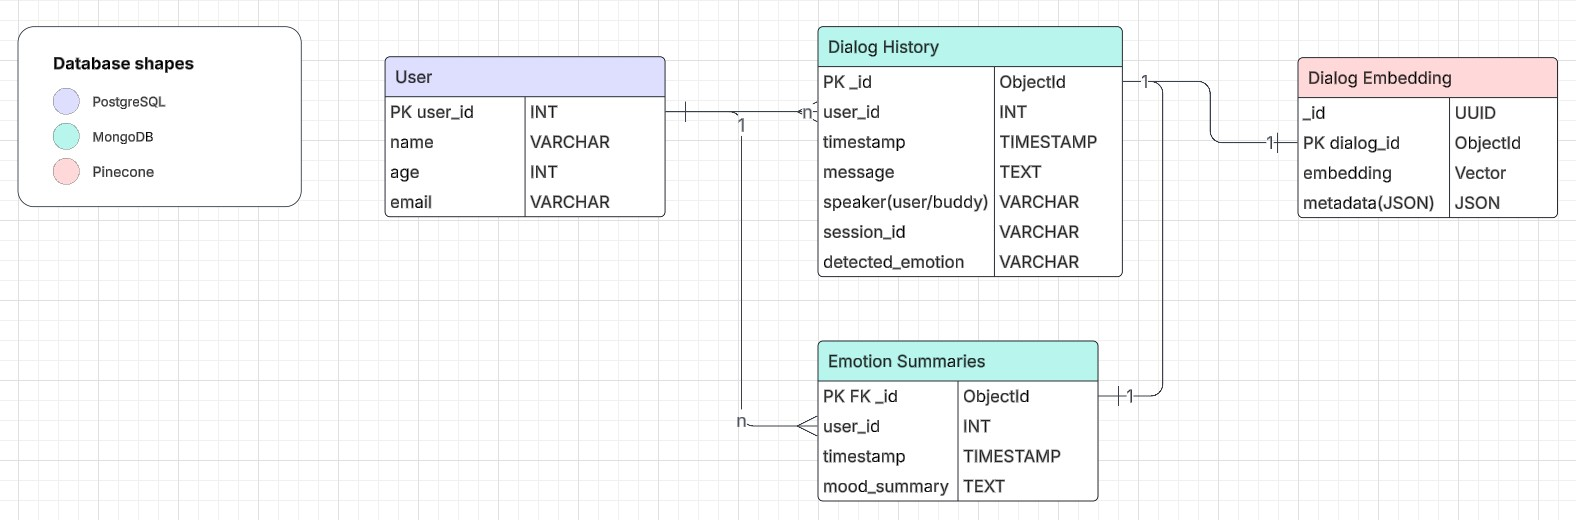
\includegraphics[width = 1.00\textwidth]{figures/ER_Diagram.png}
	\caption{\textbf ER-Diagram for the Database}
	\label{fig:ER_Diagram}
\end{figure}

\section{Hyperparameter Configurations}
\begin{itemize}
	\item Faster Whisper (Speech-to-Text):
	\begin{itemize}
		\item Model: `large-v3` (high accuracy model)
		\item Compute Type: `int8\_float16` (optimized for GPU)
		\item Device: `cuda` (GPU acceleration enabled)
		\item VAD: `WebRTCVAD` (Mode 1 for aggressive voice activity detection)
	\end{itemize}

	\item Google Text-to-Speech API:
	\begin{itemize}
		\item Voice Name: `th-TH-Chirp3-HD-Charon` (Neural2 high-definition male voice)
		\item Audio Encoding: `MP3`
		\item Language Code: `th-TH` (Thai)
	\end{itemize}
	
	\item GEMMA 3:  
	\begin{itemize}
		\item Model: `gemma3:4b` (4-billion parameter version, optimized via Ollama)
		\item Max Tokens (num\_predict): `100` (strictly limits response length for concise audio output)
		\item System Prompt: Configured for an elderly companion persona (Thai language, casual tone, no polite particles `Ka/Krub`, max 4 sentences).
		\item GPU Acceleration: `Enabled` (if running on a supported GPU)
	\end{itemize}
	
	\item ZegoCloud Video Call: 
	\begin{itemize}
		\item SDK: `zego\_uikit\_prebuilt\_call` (Flutter)
		\item Signaling: `zego\_uikit\_signaling\_plugin`
		\item Architecture: Peer-to-peer WebRTC wrapper
	\end{itemize}
\end{itemize}

\section{Performance Evaluation}

The performance of the smart companion system will be evaluated based on the following metrics:

\subsection{Emotion Recognition Accuracy}

Emotion recognition accuracy will be measured using standard classification evaluation metrics:

\begin{itemize}
	\item \textbf{Confusion Matrix}: A table comparing predicted emotions against actual labels. It consists of:
	\begin{itemize}
		\item \textbf{True Positive (TP)}: Correctly predicted positive instances.
		\item \textbf{False Positive (FP)}: Incorrectly predicted positive instances.
		\item \textbf{True Negative (TN)}: Correctly predicted negative instances.
		\item \textbf{False Negative (FN)}: Incorrectly predicted negative instances.
	\end{itemize}
	\item \textbf{Precision, Recall, and F1-Score}:
	\begin{itemize}
		\item \textbf{Precision} = $\frac{TP}{TP + FP}$
		\item Measures the proportion of correctly predicted positive instances among all predicted positive instances.
		\item \textbf{Recall} = $\frac{TP}{TP + FN}$
		\item Measures the proportion of correctly predicted positive instances among all actual positive instances.
		\item \textbf{F1-Score} = $2 \times \frac{\text{Precision} \times \text{Recall}}{\text{Precision} + \text{Recall}}$
		\item The harmonic mean of precision and recall, balancing both metrics.
	\end{itemize}
	\item \textbf{Overall Accuracy}:
	\begin{itemize}
		\item $\text{Accuracy} = \frac{TP + TN}{TP + TN + FP + FN}$
		\item Measures the overall correctness of the model by considering both positive and negative instances.
	\end{itemize}
\end{itemize}

\subsection{Dialogue Generation Quality}

The evaluation of the model's ability to generate coherent and relevant responses is primarily conducted using an "LLM-as-Judge" methodology, complemented by human evaluation. This approach leverages a superior language model to assess the semantic quality of generated text, which correlates better with human judgment than traditional n-gram metrics.

\begin{itemize}
	\item \textbf{LLM-as-Judge (Gemini-2.5-Flash)}:
	\begin{itemize}
		\item A high-capability cloud model serves as the evaluator for responses generated by the local \textbf{Gemma 3:4b} model.
		\item \textbf{Scoring Scale}: Responses are rated on a scale of 1-10.
		\item \textbf{Evaluation Dimensions}:
		\begin{itemize}
			\item \textbf{Clarity}: Measures linguistic correctness and ease of comprehension.
			\item \textbf{Relevance to Elderly}: Assesses the appropriateness of the tone and content for the target demographic.
			\item \textbf{Conciseness}: Evaluates the efficiency of information delivery, prioritizing brevity for audio output.
		\end{itemize}
	\end{itemize}
	\item \textbf{Human Evaluation}:
	\begin{itemize}
		\item \textbf{Mean Opinion Score (MOS)}: Human participants rate interactions on a 1-5 scale.
		\item \textbf{Criteria}: Coherence, Fluency, Empathy, and Overall Satisfaction.
	\end{itemize}
\end{itemize}

\subsection{Speech-to-Text (STT) Performance}

The accuracy of the Thai speech-to-text module (Faster Whisper) will be evaluated using:

\begin{itemize}
	\item \textbf{Word Error Rate (WER)}:
	\begin{itemize}
		\item $\text{WER} = \frac{S + D + I}{N}$
		\item where $S$ = substitutions, $D$ = deletions, $I$ = insertions, and $N$ = total words in reference text.
	\end{itemize}
	\item \textbf{Character Error Rate (CER)}:
	\begin{itemize}
		\item $\text{CER} = \frac{S + D + I}{N}$
		\item where $N$ represents total characters in reference text, useful for Thai language without explicit word boundaries.
	\end{itemize}
\end{itemize}


\subsection{Video Call Quality}

The reliability and quality of the real-time communication feature, powered by the ZegoCloud SDK, are assessed against industry-standard benchmarks for telecommunication.

\begin{itemize}
	\item \textbf{Connection Success Rate}: The percentage of call attempts that successfully establish a peer-to-peer connection.
	\item \textbf{Average Latency}: The end-to-end delay (measured in milliseconds) between the audio/video capture on one device and its playback on the other. This is critical for maintaining a natural conversation flow.
	\item \textbf{Call Stability}: The ability of the system to maintain a continuous connection without drops or significant quality degradation over an extended period (e.g., >10 minutes).
	\item \textbf{Packet Loss Tolerance}: The system's resilience to network instability, specifically its ability to maintain audio intelligibility and video clarity despite packet loss.
\end{itemize}

\subsection{Software Testing and Validation}

To ensure the robustness and usability of the mobile application and backend services, a comprehensive testing strategy is employed, encompassing both functional and structural verification, as well as quantitative usability assessment.

\begin{itemize}
	\item \textbf{Black Box Testing}:
	\begin{itemize}
		\item \textbf{Functional Testing}: Verifies that all application features (e.g., login, call initiation, dashboard updates) function as specified in the requirements without knowledge of the internal code structure.
		\item \textbf{User Acceptance Testing (UAT)}: Real users from the target demographic perform typical tasks to validate the system's usability and effectiveness in real-world scenarios.
	\end{itemize}
	\item \textbf{White Box Testing}:
	\begin{itemize}
		\item \textbf{Unit Testing}: Validates individual components and functions (e.g., API endpoints, database queries) to ensure they produce correct outputs for given inputs.
		\item \textbf{Integration Testing}: Verifies that different modules (e.g., the mobile app and the API server) interact correctly and data flows seamlessly between them.
	\end{itemize}
    \item \textbf{System Usability Scale (SUS)}:
    \begin{itemize}
        \item A standardized 10-item questionnaire used to assess the perceived usability of the system.
        \item Participants rate each item on a 5-point Likert scale (1 = Strongly Disagree, 5 = Strongly Agree).
        \item The final score ranges from 0 to 100, providing a global measure of system usability, where a score above 68 is typically considered "above average".
    \end{itemize}
\end{itemize}
